\documentclass{article}
\usepackage{graphicx} % Required for inserting images
\usepackage[labelformat=empty]{caption}
\usepackage{hyperref}
\usepackage[top=1.0in, bottom=1.0in]{geometry}
\usepackage{enumitem}
\graphicspath{ {./images/} }
\date{}

\title{CS 699 - Project\\ Bird Image Classification and Visualization}


\begin{document}

\maketitle

\section{Image Classification}

\noindent Uploaded image:

\begin{figure}[h!]
\centering
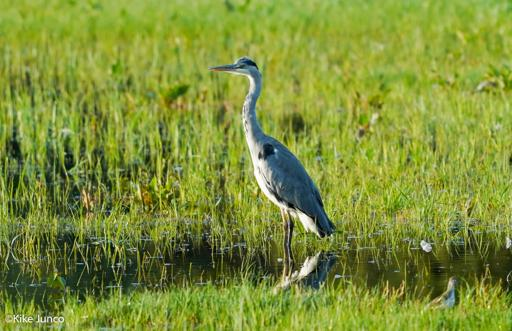
\includegraphics[width=100mm]{bird_test}
\caption*{Prediction: modelpredictedspecies}
\label{fig:method}
\end{figure}

\noindent Classifier: classifiername
\newline
\newline
\newline
\noindent Top 5 predictions:
\newline
\begin{table}[h!]
\centering
\begin{tabular}{|c|c|c|} 
\hline
 S.No. & Species Name & Prediction Probability\\ 
\hline
 1 & Blue Jay & probscore1 \\ 
 \hline
 2 & Grey Heron & probscore2 \\  
 \hline
 3 & Indian Peafowl & probscore3 \\    
 \hline
 4 & Little Egret & probscore4 \\    
 \hline
 5 & Red-Vented Bulbul & probscore5 \\    
 \hline
\end{tabular}
\caption{Species wise prediciton probability}
\label{table:data}
\end{table}




\newpage
\section{Model Report}

\textbf{Classifier:} classifiername
\newline

\noindent \textbf{Dataset:}
Images scrapped from \href{https://ebird.org/explore}{eBird Portal}  for species classification across 5 species.
\newline
Total images: 5000
\newline
Train-Test Split: 80:20
\newline
\newline
\noindent \textbf{Species:}
\begin{enumerate}[noitemsep]
  \item Blue Jay
  \item Grey Heron
  \item Indian Peafowl
  \item Little Egret
  \item Red-Vented Bulbul
\end{enumerate}
\vspace{10mm}
\noindent \textbf{Metrics:}
\newline
\newline
\noindent \textbf{Classification Report:}

sklearnreport
\newline

\noindent \textbf{Confusion Matrix:}

\begin{figure}[h!]
\centering
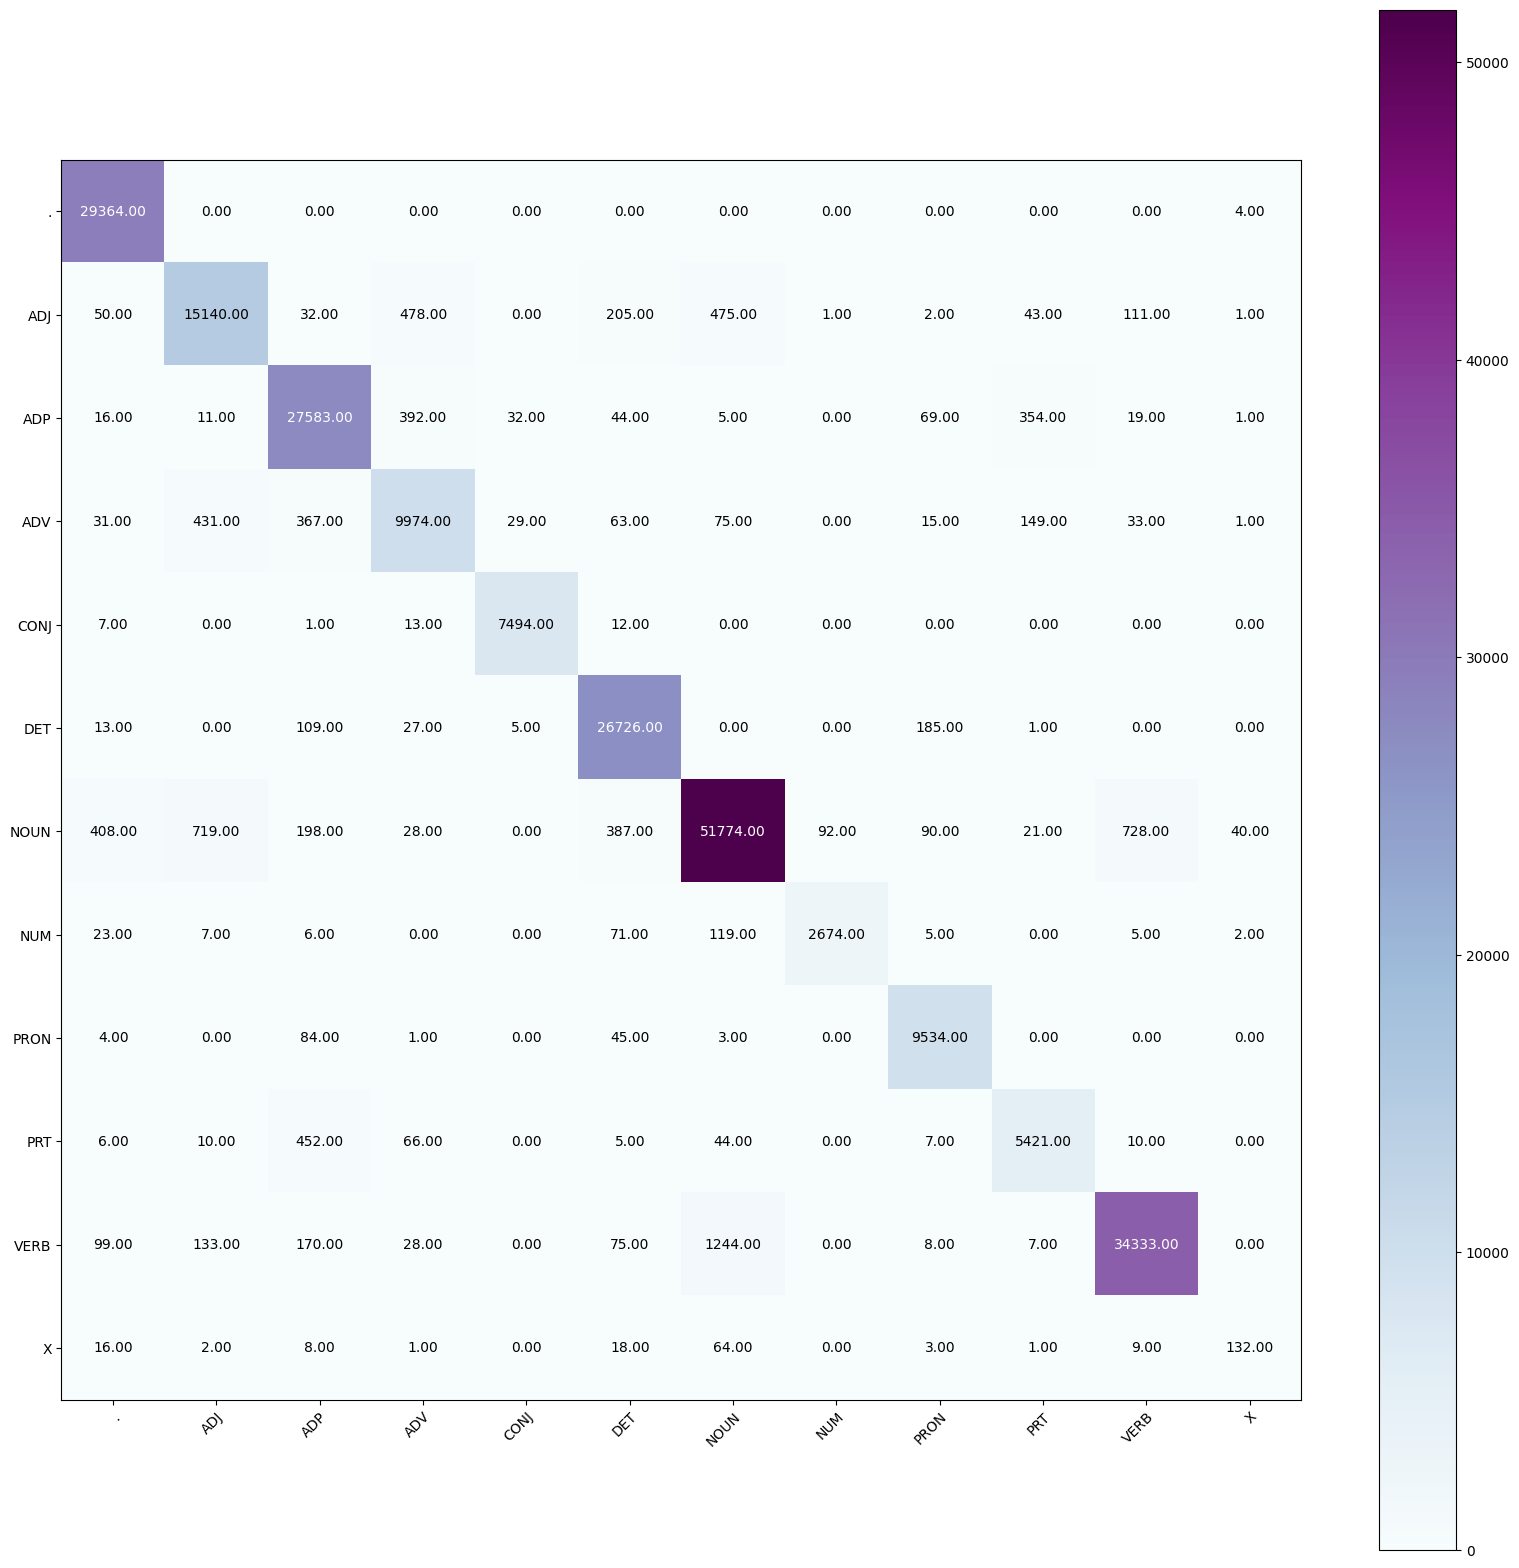
\includegraphics[width=100mm]{images/output.jpg}
\end{figure}




\end{document}
